\section{Architecture}
MyMoodle is an extension of Moodle and can be seen as a package of plugins. 
The architecture does not specify how each plugins should be created but specify a general structuring of the parts of the system. 
The complete architecture can be seen in \figref{fig:architecture}.
\begin{figure}
	\centering
		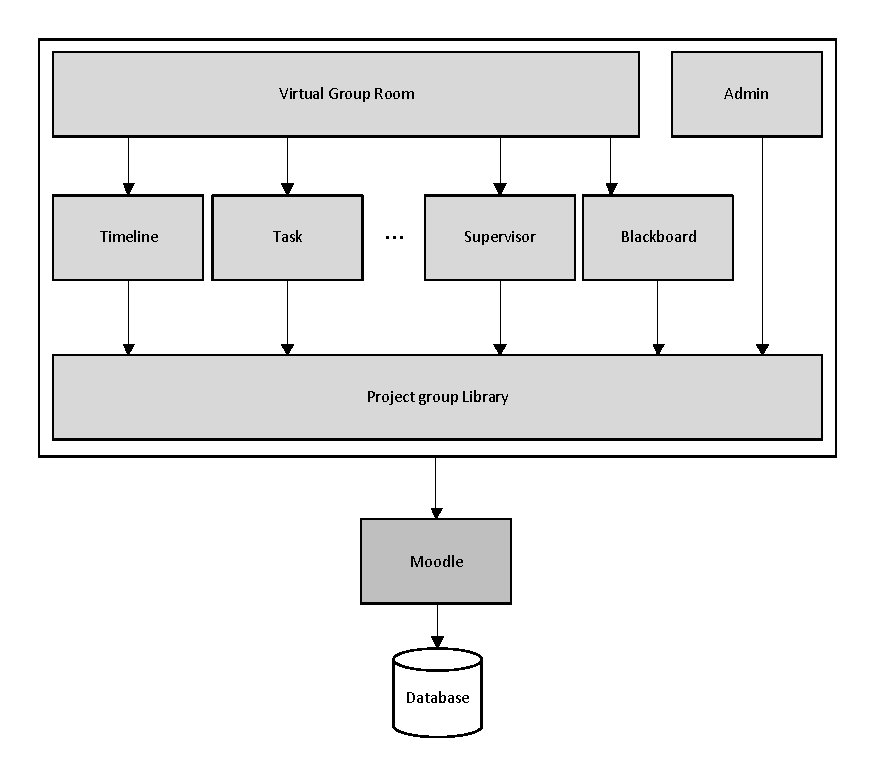
\includegraphics{images/architecture.pdf}
	\morscaption{The overall architecture of MyMoodle}
	\label{fig:architecture}
\end{figure}
The surrounding box illustrates a common dependency on the Moodle platform. 
Every part, except for the database, is dependent on Moodle to work. 
The system consists of a total of five layers. 
The three uppermost is what we implement in this project while the lowest two existed prior to the project. 
The database is extended but otherwise are these two layers unchanged.
The upper most layer is the project group view and the administration tool.
The project group view is used for presenting the project group room, described in \secref{sec:projectgroup}, and the administration tool, described in \secref{sec:projectgroupadministration}, is a tool used by managing personal for creating, editing, and deleting groups. 
Directly below the upper most layer is the ``middle'' layer which consist of the four parts: Timeline, Task, Supervisor, and Blackboard. These four parts are created by the other groups and are not explained. 
Below the middle layer is the project group library which contain common functionality.
 

There are two primary factors for creating an layered architecture. First is that we are four groups working together, which creates the need for a structured way of dependency among the groups and it lets every group know how their part is connected to the rest of the project. 
Second is that the project should be passed on and with a good architecture the comprehensibility of the project is increased thereby enhancing the likelihood of a good pass on.
It is not possible to make a strict layered architecture due to the Moodle dependency and the administration tool which does not have use the intermediate layer, but depends directly on the project group library.














